\documentclass[twocolumn,english]{article}
\usepackage[latin9]{inputenc}
\usepackage[landscape]{geometry}
\geometry{verbose,tmargin=0.5in,bmargin=0.75in,lmargin=0.5in,rmargin=0.5in}
\setlength{\parskip}{0bp}
\setlength{\parindent}{0pt}
\usepackage{float}
\usepackage{booktabs}
\usepackage{graphicx}

\makeatletter

\providecommand{\tabularnewline}{\\}




\usepackage{array}
\usepackage{multirow}
\usepackage{amsbsy}




\providecommand{\tabularnewline}{\\}

\setlength{\columnsep}{0.25in}
\usepackage{xcolor}
\usepackage{textcomp}
\usepackage{listings}
\lstset{
  tabsize=2,
  basicstyle=\small\ttfamily,
}



\usepackage{babel}
\usepackage{listings}
\renewcommand{\lstlistingname}{Listing}

\AtBeginDocument{
  \def\labelitemii{\(\bullet\)}
}

\makeatother

\usepackage{babel}
\begin{document}

\title{Reference Sheet for C211 Operating Systems}

\date{Spring 2018}
\maketitle

\paragraph{Operating systems}

have to
\begin{itemize}
\item \emph{Manage resources}: processors, memory, IO, clocks, interrupt
controllers, storage.
\item \emph{Provide clean interfaces}: offer level of abstraction above
hardware.
\end{itemize}

\paragraph{Flavours}

E.g. server / supercomputer / smartphone / embedded operating systems.

\paragraph{Kernel}

Part of the OS that:
\begin{itemize}
\item Is always loaded in memory.
\item Executes in a privileged mode with access to all hardware.
\end{itemize}

\paragraph{Structure}
\begin{itemize}
\item \emph{Monolithic kernels}: single executable with its own address
space.
\begin{itemize}
\item $+$ Efficient calls within kernel.
\item $+$ Easier to write components due to shared memory.
\item $-$ Complex design with lots of interactions.
\item $-$ No protection between kernel components.
\end{itemize}
\item \emph{Microkernels}: minimal level kernel with functionality in user-level
servers.
\begin{itemize}
\item $+$ Kernel not complex so less error prone.
\item $+$ Servers have clean interfaces.
\item $+$ Servers can crash and restart without crashing kernel.
\item $-$ Overhead of IPC within kernel high.
\end{itemize}
\item \emph{Hybrid kernels}: combines features of each. Compromise between
clean design and performance overhead.
\end{itemize}

\section{Processes}

\paragraph{Process}

An instance of a program being executed.
\begin{itemize}
\item Provides illusion of concurrency.
\item Provides isolation between programs (each has its own address space).
\item Simplicity of programming (can assume complete control).
\item Allows better utilisation of resources.
\end{itemize}

\paragraph{Types of Concurrency}
\begin{itemize}
\item \emph{Pseudo concurrency}: single processor is switched between processes
by interleaving (e.g. by \emph{time-slicing}).
\item \emph{Real concurrency}: utilises multiple physical processors.
\end{itemize}

\paragraph{CPU Utilisation}

If we have $n$ processes, each with probability $p$ of waiting for
I/O at any time, expect CPU utilisation to be $1-p^{n}$.

\paragraph{Context Switch}

Processor switches from executing process $A$ to process $B$.
\begin{itemize}
\item OS may make scheduling decisions: may switch processes in response
to events/interrupts.
\item Adds non-determinism to execution (events occur in unpredictable order).
\item \emph{Expensive}: need to save/restore state, lost CPU caches (including
TLBs), ...
\end{itemize}

\paragraph{Process Control Block}

Each process has a \emph{process descriptor} or \emph{process control
block}, kept in the \emph{process table}.
\begin{itemize}
\item Process has its own virtual machine (CPU, address space, file descriptors,
...).
\item Need to store state:
\begin{itemize}
\item \emph{Registers}: PC, page table register, stack pointer, ...
\item \emph{Process management info}: ID, parent, group, priority, CPU used,
...
\item \emph{File management info}: root directory, working directory, open
FDs
\end{itemize}
\end{itemize}

\paragraph{Process Types}
\begin{itemize}
\item \emph{Foreground processes}: interact with users.
\item \emph{Background processes}: daemons.
\end{itemize}

\paragraph{Process Creation}

Can happen by system initialisation, user requests, system calls.

\paragraph{Process termination}
\begin{itemize}
\item \emph{Normal completion}: process completes execution of body.
\item \emph{System call}: call to \texttt{exit()}.
\item \emph{Abnormal exit}: run into error / unhandled exception.
\item \emph{Never}: e.g. (hopefully) web servers.
\end{itemize}

\paragraph{Process Hierarchies}

All processes form a process tree with \texttt{init} as the root (\emph{process
group}).

\paragraph{Creation and Termination}
\begin{itemize}
\item \texttt{fork()} creates a new child process with an exact copy of
parent. 
\begin{itemize}
\item In parent process, returns PID of child.
\item In child process, returns 0.
\end{itemize}
\item \texttt{execve(path, argv, envp)} executes a command.
\item \texttt{waitpid(pid, stat, option)} suspends execution of calling
process until \texttt{pid} terminates normally or a signal is received.
\begin{itemize}
\item \texttt{-1} waits for any child.
\item \texttt{0} waits for any child in the same process group as the caller.
\item \texttt{-gid} waits for any child with process group \texttt{gid}.
\end{itemize}
\item \texttt{exit(status)} terminates process (called implicitly).
\item \texttt{kill(pid, sig)} sends signal \texttt{sig} to \texttt{pid}.
\end{itemize}

\paragraph{Communicating between Processes}

Files, signals, pipes, message queues, sockets, shared memory, semaphores.

\paragraph{UNIX Signals}

Used to notify processes when an event occurs.
\begin{itemize}
\item User ID of the receiving process must match that of the sending process
or have appropriate privileges.
\item Kernel can send signal to any process.
\item \texttt{SIGFPE} division by 0, \texttt{SIFSEGV} segment violation,
\texttt{SIGPIPE} writes to closed pipe, \texttt{SIGINT} interrupted
process, ....
\item Process can ignore / handle signals (except \texttt{SIGKILL} and \texttt{SIGSTOP}).
\end{itemize}

\paragraph{UNIX Pipes}

Connects standard output of one process to standard input of another.
Allows \emph{one-way} communication.
\begin{itemize}
\item \texttt{pipe(fd{[}2{]})}: \texttt{fd{[}0{]}} is the read end and \texttt{fd{[}1{]}}
the write end of the pipe.
\item \emph{Named pipes} (FIFOs): persistent pipes that outlive process
which created them.
\begin{itemize}
\item Stored on the filesystem, but more efficient since it only exists
in memory.
\end{itemize}
\end{itemize}

\section{Threads}

Execution streams that share the same address space (each process
can contain one or more threads).

\begin{table}[H]
\centering{}%
\begin{tabular}{cc}
\toprule 
\textbf{Per process} & \textbf{Per thread}\tabularnewline
\midrule
Address space & PC\tabularnewline
Global variables & Registers\tabularnewline
Open files & Stack\tabularnewline
Child processes & \tabularnewline
Signals & \tabularnewline
\bottomrule
\end{tabular}
\end{table}

\paragraph{Uses}

Applications with multiple activities which:
\begin{enumerate}
\item Execute in parallel.
\item Access and process the same data.
\item May sometimes block.
\end{enumerate}
Processes are more heavyweight (difficult communication and expensive
creation / context switching / termination).

\paragraph{PThreads}
\begin{itemize}
\item \texttt{pthread\_create(thread, attr, start\_routine, arg)} creates
a new thread.
\item \texttt{pthread\_exit(value\_ptr)} terminates thread and makes \texttt{value\_ptr}
available to any join. Called implicitly when thread returns.
\begin{itemize}
\item If \texttt{main()} terminates, entire process is terminated, unless
\texttt{pthread\_exit()} is called (process executes until last thread
terminates or \texttt{exit()} is called).
\end{itemize}
\item \texttt{pthread\_yield()} releases CPU to let another thread run.
\item \texttt{pthread\_join(thread, value\_ptr)} blocks until thread terminates.
\end{itemize}

\paragraph{Implementation Options}
\begin{itemize}
\item \emph{User-level}: kernel is not aware of threads, each process manages
its own threads.
\begin{itemize}
\item Implemented by software library.
\item Process maintains \emph{thread table} for \emph{thread scheduling}.
\item $+$ Better performance (creation, termination, switching and joining
are fast since no kernel involvement required).
\item $+$ Each application can have its own scheduling algorithm.
\item $-$ Blocking system calls stops all threads in process. Non-blocking
I/O can be used (difficult to use).
\item $-$ During page fault, OS blocks whole process.
\end{itemize}
\item \emph{Kernel-level}: managed by the kernel.
\begin{itemize}
\item $+$ Blocking system calls / page faults are easily accommodated.
\item $-$ Thread creation and termination requires system calls so more
expensive (can use \emph{thread pools} to recycle threads).
\item $-$ Thread synchronisation requires blocking system calls so more
expensive.
\item $-$ Thread switching requires system calls so more expensive.
\item $-$ No application-specific schedulers.
\end{itemize}
\item \emph{Hybrid approach}: use kernel threads and multiple user-level
threads onto kernel-threads.
\end{itemize}

\section{Scheduling}

\begin{figure}[H]
\centering{}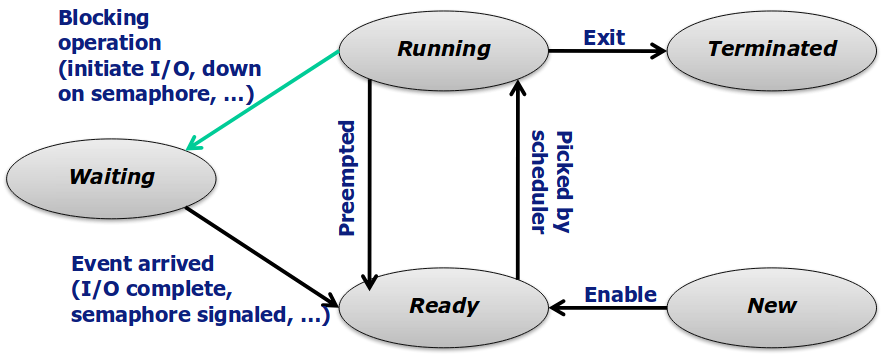
\includegraphics[width=0.75\linewidth]{img/process-states}
\end{figure}

\paragraph{Goals}
\begin{itemize}
\item Ensure fairness.
\item Avoid indefinite postponement.
\item Enforce policy (e.g. priorities).
\item Maximise resource utilisation (e.g. CPU, I/O devices).
\item Minimise overhead (from scheduling decisions and context switches).
\end{itemize}
\rule{0.25\columnwidth}{0.5pt}
\begin{itemize}
\item Batch systems: optimise for \emph{throughput} and \emph{turnaround
time}.
\item Interactive systems: optimise for \emph{response time}.
\item Real-time systems: meet deadlines.
\end{itemize}

\paragraph{Preemption}
\begin{itemize}
\item \emph{Non-preemptive}: let process run until it blocks or voluntarily
releases CPU.
\item \emph{Preemptive}: Let process run for a maximum amount of fixed time,
using clock interrupt.
\end{itemize}

\paragraph{Processes}
\begin{itemize}
\item \emph{CPU-bound}: spend most of their time using the CPU.
\item \emph{I/O-bound}: spend most of their time waiting for I/O and use
CPU only briefly.
\end{itemize}

\subsection{Scheduling Algorithms}

\paragraph{First-Come-First-Served}

Non-preemptive. Runnable process added to the end of ready queue.
\begin{itemize}
\item $+$ No indefinite postponement (all processes are eventually scheduled).
\item $+$ Really easy to implement.
\item $-$ Poor turnaround time if a long job is followed by many short
jobs.
\end{itemize}

\paragraph{Round Robin}

Run process until it blocks or time quantum exceeded.
\begin{itemize}
\item $+$ Fair: ready jobs get equal share of the CPU.
\item $+$ Good response time for small number of jobs.
\item $+$ Average turnaround time is low when run-times differ.
\item $+$ Average turnaround time is poor for similar run-times.
\end{itemize}
As quantum increases:
\begin{itemize}
\item $+$ Overhead decreases.
\item $-$ Response time worsens.
\end{itemize}
Quantum value should be:
\begin{itemize}
\item Much large than cost of a context switch,
\item But provide decent response time.
\end{itemize}

\paragraph{Shortest Job First}

Non-preemptive scheduling with run-times known in advance. Pick shortest
job first.
\begin{itemize}
\item $-$ Run-times not usually known in advance.
\begin{itemize}
\item Heuristics not always applicable.
\item User-supplied estimates encourage cheating (terminate processes if
they exceed estimate).
\end{itemize}
\end{itemize}

\paragraph{Shortest Remaining Time}

Preemptive version of shortest job first.

\paragraph{Fair-Share}

Round robin taking into account user that owns a process.

\paragraph{Lottery Scheduling}
\begin{itemize}
\item Jobs receive lottery tickets for various resources (e.g. CPU time).
\item At each scheduling decision, one ticket is chosen at random.
\item $+$ Highly responsive.
\item $+$ No starvation.
\item $+$ Jobs can exchange tickets (allows for priority donation, jobs
can cooperate).
\item $+$ Adding / removing jobs affect remaining jobs proportionally.
\item $-$ Unpredictable response time.
\end{itemize}

\subsection{Priority Scheduling}

Always run the job with the highest priority.
\begin{itemize}
\item Priorities could be externally defined or on some process-specific
metrics.
\item Priorities could be static or dynamic.
\end{itemize}

\paragraph{General-Purpose Scheduling}
\begin{itemize}
\item Favour short and I/O bound jobs.
\item Quickly determine the nature of the job and adapt to changes.
\end{itemize}

\paragraph{Multilevel Feedback Queues}

One queue for each priority level.
\begin{itemize}
\item Run job on highest non-empty priority queue.
\item Each queue can use a different scheduling algorithm (usually round
robin).
\item Need to worry about starvation of low-priority jobs:
\begin{itemize}
\item Recompute priorities periodically (e.g. based on how much CPU they've
used).
\item \emph{Ageing}: increase job's priority as it waits.
\end{itemize}
\item $-$ Not very flexible, priorities make no guarantees.
\item $-$ Does not react quickly to changes - often needs warm-up period.
\item $-$ Cheating is still a concern.
\item $-$ Cannot donate priority.
\end{itemize}

\section{Synchronisation}

\section{Deadlocks}

\section{Memory Management}

\section{Device Management}

\section{Disk Management}

\section{File Systems}

\section{Security}
\end{document}
